\section{Vivado工程实现}

\subsection{工程创建}

\begin{enumerate}[leftmargin=2em]
    \item 打开Vivado，选择 Create Project，项目类型为 RTL Project。
    \item 目标器件选择 Artix-7 系列，型号为 \texttt{xc7a100tcsg324-1}。
\end{enumerate}

\subsection{源文件添加}

将21个Verilog设计源文件添加到工程中，设置 \texttt{openmips\_board} 为顶层模块。同时添加引脚约束文件 \texttt{openmips.xdc}。

\subsection{指令ROM IP核生成}

使用MARS汇编器将测试程序编译为机器码，导出为二进制文本格式后转换为COE文件，用于初始化Distributed Memory Generator IP核。

\begin{figure}[H]
    \centering
    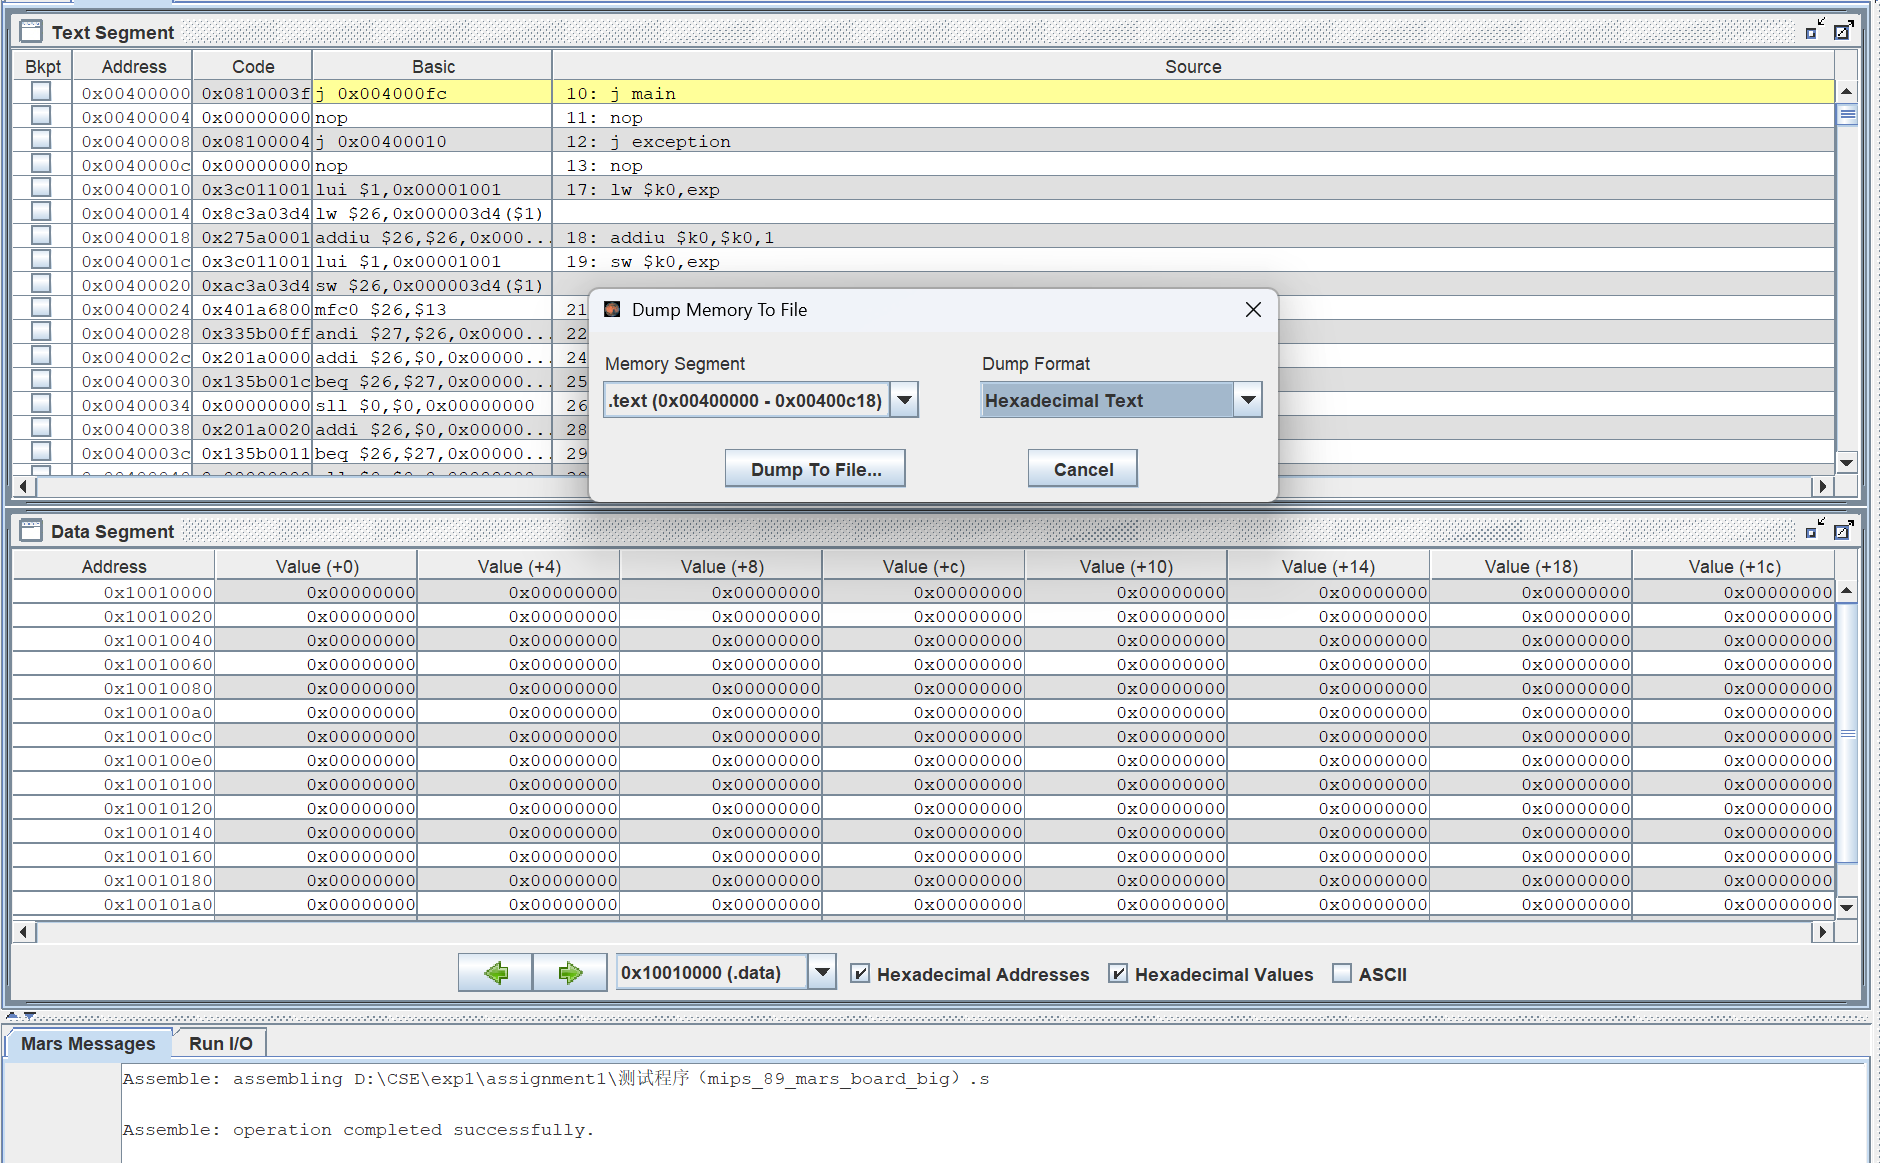
\includegraphics[width=0.8\textwidth]{img/mars_export.png}
    \caption{MARS汇编器导出机器码}
\end{figure}

IP核配置参数：
\begin{itemize}[leftmargin=2em]
    \item 名称：\texttt{inst\_rom\_for\_cpu89}
    \item 深度：2048
    \item 数据宽度：32位
    \item 类型：ROM
    \item 输入/输出选项：Non Registered
\end{itemize}

\begin{figure}[H]
    \centering
    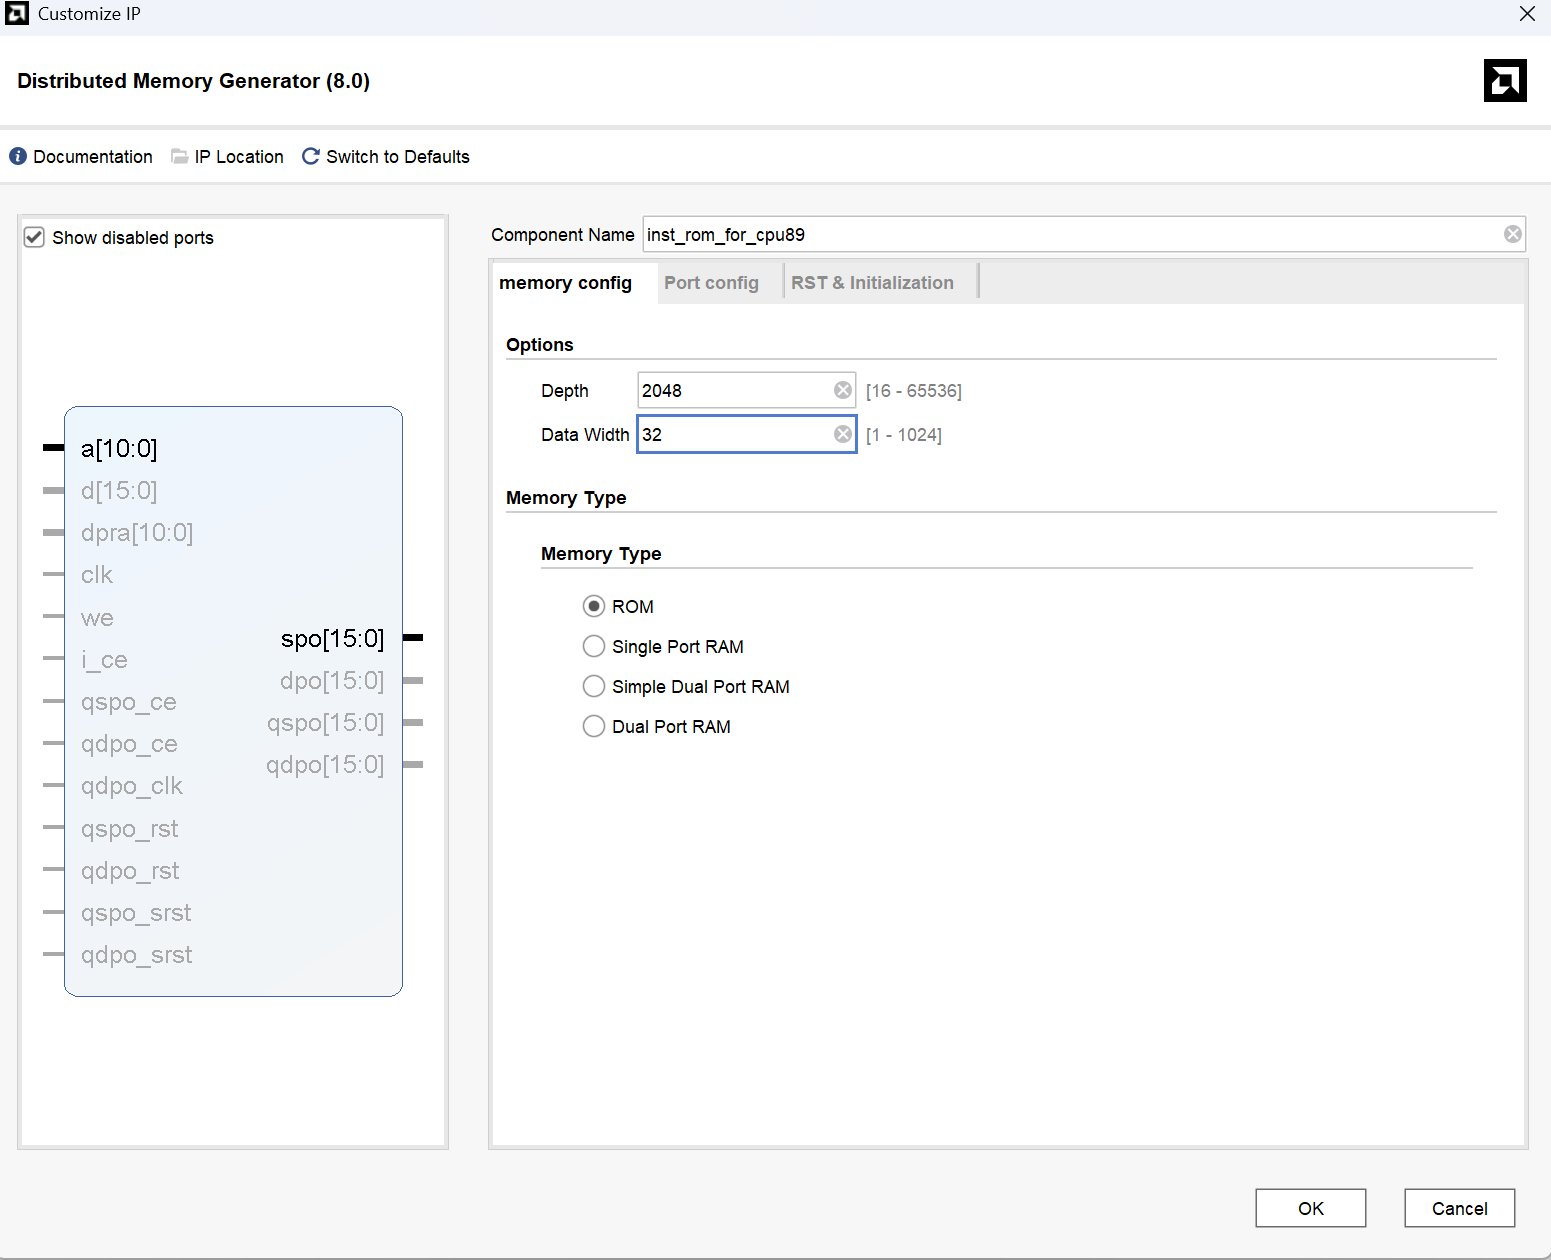
\includegraphics[width=0.8\textwidth]{img/ip_core_generate.png}
    \caption{Distributed Memory Generator IP核生成}
\end{figure}

\subsection{引脚分配}

\begin{table}[H]
    \centering
    \caption{FPGA引脚分配}
    \begin{tabular}{lll}
        \toprule
        \textbf{信号} & \textbf{引脚} & \textbf{功能说明} \\
        \midrule
        \texttt{clk\_in} & E3 & 100MHz板载时钟输入 \\
        \texttt{reset} & N17 & 复位按钮（BTNC） \\
        \texttt{en\_clk} & V10 & 时钟模式选择开关 \\
        \texttt{choose[0]} & J15 & 显示选择开关（低位） \\
        \texttt{choose[1]} & L16 & 显示选择开关（高位） \\
        \texttt{o\_seg[7:0]} & T10,R10,K16,K13,P15,T11,L18,H15 & 七段数码管段选 \\
        \texttt{o\_sel[7:0]} & J17,J18,T9,J14,P14,T14,K2,U13 & 七段数码管位选 \\
        \bottomrule
    \end{tabular}
\end{table}

所有I/O引脚电平标准设置为 LVCMOS33。

\subsection{综合与实现}

\begin{enumerate}[leftmargin=2em]
    \item \textbf{综合（Synthesis）}：将Verilog代码转换为门级网表。
    \item \textbf{实现（Implementation）}：完成布局布线，将逻辑映射到FPGA具体资源。
    \item \textbf{生成比特流（Generate Bitstream）}：生成可下载到FPGA的配置文件。
\end{enumerate}


